% !TEX root = ../main.tex
\paragraph{Forward Time-of-Flight (FTOF)}
    \begin{wrapfigure}{r}{0.50\textwidth}
        \centering\frame{
        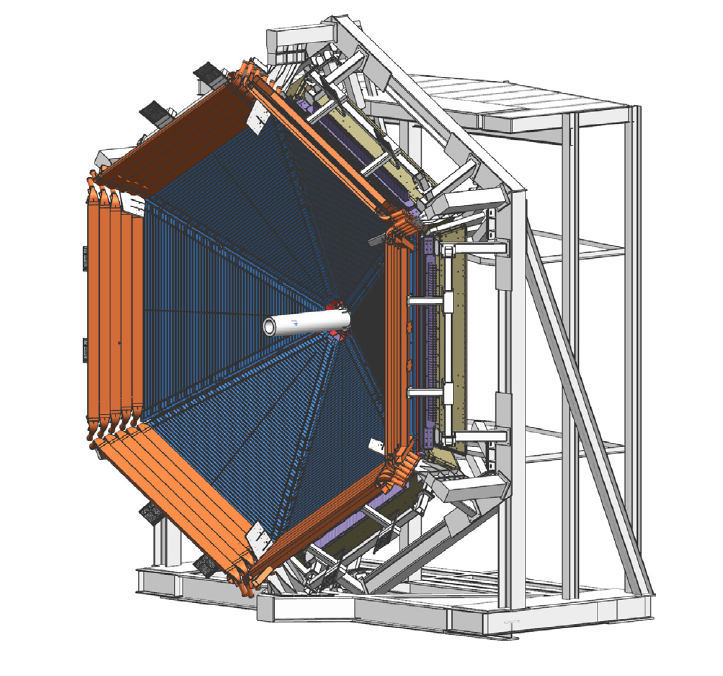
\includegraphics[width=\linewidth]{11experiment/img/214ftof.png}}
        \caption[FTOF]{Render of the Forward Carriage with the FTOF system showing the panel-1b counters on the inside (dark blue), and the panel-2 counters on the outside (bronze).
        The panel-1a counters are located immediately downstream of the panel-1b counters and are not visible in the render.
        Part of the PCAL is visible downstream of the FTOF panels.}
        \label{fig::ftof}
    \end{wrapfigure}

    The FTOF system is used to measure the TOF of charged particles emerging from the target during beam operation.
    It includes six sectors of plastic scintillators with double-sided PMT readout.
    Each sector consists of three arrays of counters separated in panels, with panel-1a having 23 counters, panel-1b 62 counters, and panel-2 5 counters.
    The system is required to get excellent timing resolution required for particle identification and good segmentation to get flexible triggering options.

    The detectors span a range in polar angle from $5\degree$ to $45\degree$, covering $50\%$ in the azimuth at $5\degree$ and $90\%$ at $45\degree$.
    The lengths of the counters range from $32.3 ~\text{cm}$ to $376.1 ~\text{cm}$ in panel 1a, from $17.3 ~\text{cm}$ to $407.9 ~\text{cm}$ in panel-1b, and from $371.3 ~\text{cm}$ to $426.2 ~\text{cm}$ in panel-2.
    The average timing resolution in panel-1a is $125 ~\text{ps}$, $85 ~\text{ps}$ in panel-1b, and $155 ~\text{ps}$ in panel-2 \cite{carman2020ftof}.
    A render of the detector can be seen in Figure \ref{fig::ftof}.
